\documentclass[10pt]{beamer}
\usepackage[english]{babel}
\usepackage[utf8]{inputenc}
\usepackage[T1]{fontenc}
\usepackage{helvet}

%-------------------------------------------------------
% INFORMATION IN THE TITLE PAGE
%-------------------------------------------------------

\newcommand{\cstitle}{\textbf{Tópicos en Computación Gráfica}}
\subtitle[]{Final project proposal}
\newcommand{\cscourseCode}{Tópicos en Computación Gráfica}
\newcommand{\csauthor}{MSc. Vicente Machaca Arceda}
\institute[UNSA]{Universidad Nacional de San Agustín}
\newcommand{\csemail}{vmachacaa@unsa.edu.pe}
\newcommand{\instituteabr}{UNSA}
\newcommand{\nameUp}{}
\date{2021}
\title[\cscourseCode]{\cstitle}
\author{\csauthor}
%%%%%%%%%%%%%%%%%

%-------------------------------------------------------
% CHOOSE THE THEME
%-------------------------------------------------------
\def\mycmd{0} % CS THEME
\def\mycmd{1} % MYTHEME
%-------------------------------------------------------

\if\mycmd1
	\usetheme[]{Feather}
	\newcommand{\chref}[2]{	\href{#1}{{\usebeamercolor[bg]{Feather}#2}} }
\else
	\usepackage{csformat}
	\newcommand{\chref}[3][blue]{\href{#2}{\color{#1}{#3}}}%
\fi

\newcommand{\1}{
        	\setbeamertemplate{background}{
        		
\includegraphics[width=\paperwidth,height=\paperheight]{img/1}
        		\tikz[overlay] \fill[fill opacity=0.75,fill=white] (0,0) rectangle (-\paperwidth,\paperheight);
        	}
}



%-------------------------------------------------------
% THE BODY OF THE PRESENTATION
%-------------------------------------------------------

\begin{document}


\AtBeginSubsection[]
{
    \begin{frame}
        \frametitle{Overview}
        \tableofcontents[currentsubsection]
    \end{frame}
}


%-------------------------------------------------------
% THE TITLEPAGE
%-------------------------------------------------------

\if\mycmd1 % MY THEME
	\1{
	\begin{frame}[plain,noframenumbering] 
		\titlepage 
	\end{frame}}

\else % CS THEME
	\maketitle
\fi


%-------------------------------------------------------
%-------------------------------------------------------
\begin{frame}{Content}
	\tableofcontents
\end{frame}
%-------------------------------------------------------
%-------------------------------------------------------


%%%%%%%%%%%%%%%%%%%%%%%%%%%%%%%%%%%%%%%%%%%%%%%%%%%%%%%%%%%%%%%%%%%%%%%%%%%%%%%%%%%%%%%%%%%%%%%%%%%%%%%%%%%%%%%%
%%%%%%%%%%%%%%%%%%%%%%%%%%%%%%%%%%%%%%%%%%%%%%%%%%%%%%%%%%%%%%%%%%%%%%%%%%%%%%%%%%%%%%%%%%%%%%%%%%%%%%%%%%%%%%%%
%%%%%%%%%%%%%%%%%%%%%%%%%%%%%%%%%%%%%%%%%%%%%%%%%%%%%%%%%%%%%%%%%%%%%%%%%%%%%%%%%%%%%%%%%%%%%%%%%%%%%%%%%%%%%%%%
\section{Introduction}
%%%%%%%%%%%%%%%%%%%%%%%%%%%%%%%%%%%%%%%%%%%%%%%%%%%%%%%%%%%%%%%%%%%%%%%%%%%%%%%%%%%%%%%%%%%%%%%%%%%%%%%%%%%%%%%%
%%%%%%%%%%%%%%%%%%%%%%%%%%%%%%%%%%%%%%%%%%%%%%%%%%%%%%%%%%%%%%%%%%%%%%%%%%%%%%%%%%%%%%%%%%%%%%%%%%%%%%%%%%%%%%%%
%%%%%%%%%%%%%%%%%%%%%%%%%%%%%%%%%%%%%%%%%%%%%%%%%%%%%%%%%%%%%%%%%%%%%%%%%%%%%%%%%%%%%%%%%%%%%%%%%%%%%%%%%%%%%%%%

%%%%%%%%%%%%%%%%%%%%%%%%%%%%%%%%%%%%%%%%%%%%%%%%%%%%%%%%%%%%%%%%%%%%%%%%%%%%%%%%%%%%%%%%%%%%%%%%%%%%%%%%%%%%%%%%
%%%%%%%%%%%%%%%%%%%%%%%%%%%%%%%%%%%%%%%%%%%%%%%%%%%%%%%%%%%%%%%%%%%%%%%%%%%%%%%%%%%%%%%%%%%%%%%%%%%%%%%%%%%%%%%%
%%%%%%%%%%%%%%%%%%%%%%%%%%%%%%%%%%%%%%%%%%%%%%%%%%%%%%%%%%%%%%%%%%%%%%%%%%%%%%%%%%%%%%%%%%%%%%%%%%%%%%%%%%%%%%%%
\subsection{Definitions}
%%%%%%%%%%%%%%%%%%%%%%%%%%%%%%%%%%%%%%%%%%%%%%%%%%%%%%%%%%%%%%%%%%%%%%%%%%%%%%%%%%%%%%%%%%%%%%%%%%%%%%%%%%%%%%%%
%%%%%%%%%%%%%%%%%%%%%%%%%%%%%%%%%%%%%%%%%%%%%%%%%%%%%%%%%%%%%%%%%%%%%%%%%%%%%%%%%%%%%%%%%%%%%%%%%%%%%%%%%%%%%%%%
%%%%%%%%%%%%%%%%%%%%%%%%%%%%%%%%%%%%%%%%%%%%%%%%%%%%%%%%%%%%%%%%%%%%%%%%%%%%%%%%%%%%%%%%%%%%%%%%%%%%%%%%%%%%%%%%

%-------------------------------------------------------
%-------------------------------------------------------
\begin{frame}{Definitions}{}	
	
	\begin{columns}
		\begin{column}{0.48\textwidth}
			
			\begin{block}{}
				\textbf{Proteomics} is the large-scale study of proteins \cite{anderson1998proteome}
			\end{block}
		
			\begin{block}{}
				\textbf{Proteins} are large, complex molecules that play many critical roles in the body. They do most of the work in cells. \cite{anderson1998proteome}
			\end{block}

		\end{column}
	
		\begin{column}{0.48\textwidth}
		
			\begin{figure}
				\centering
				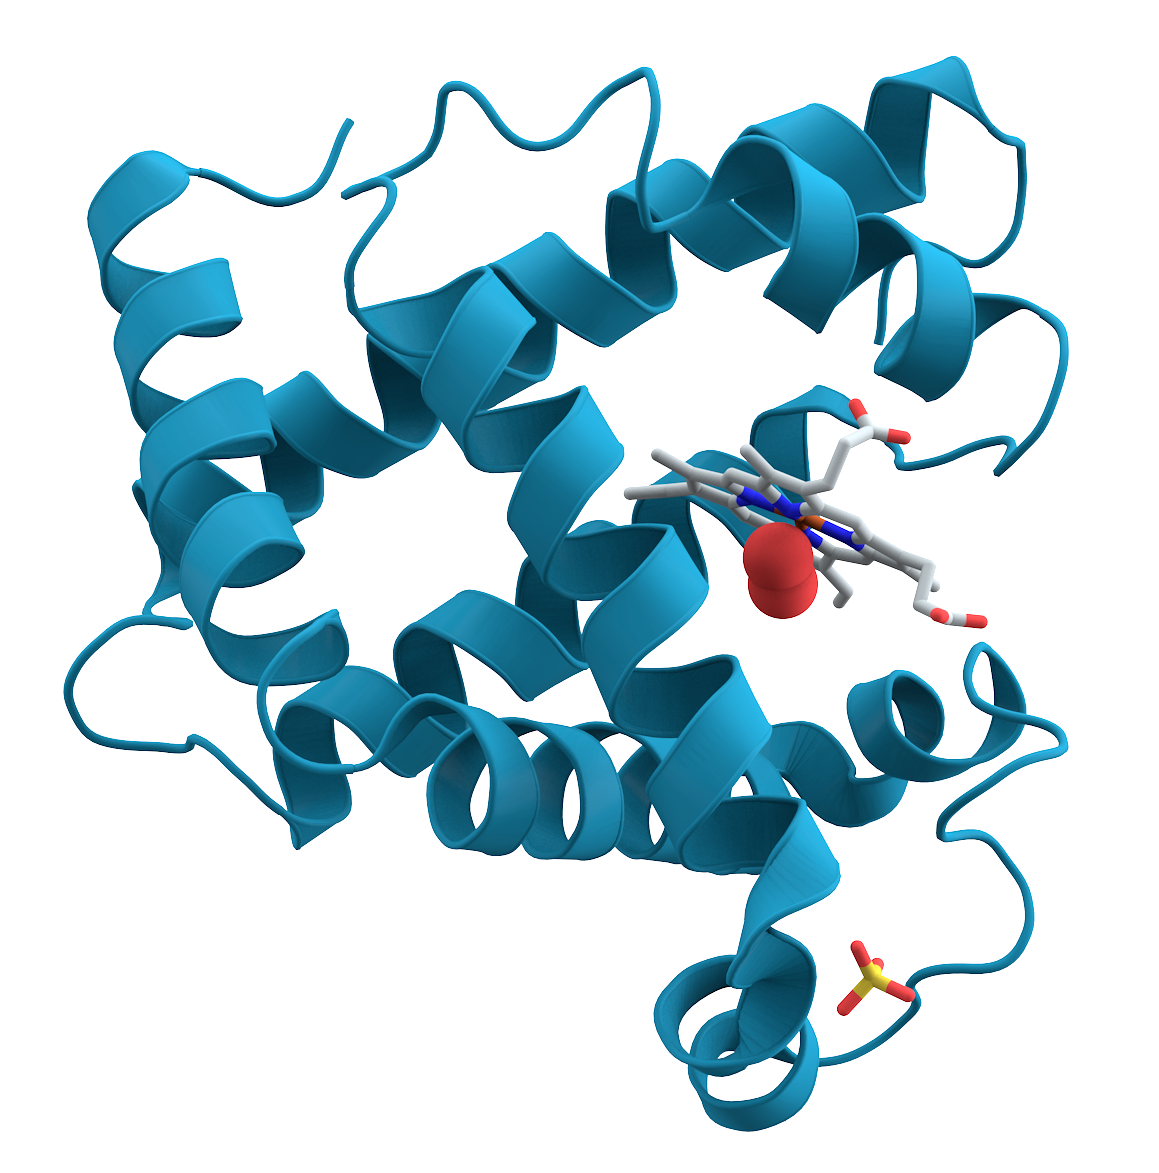
\includegraphics[width=5cm]{img/papers/myoglobin}
				\caption{A representation of the 3D structure of the protein myoglobin. Source: \chref{https://pdb101.rcsb.org/motm/1}{PDB}.}
			\end{figure}	
		
		\end{column}
	\end{columns}	
		
\end{frame}
%-------------------------------------------------------
%-------------------------------------------------------

%-------------------------------------------------------
%-------------------------------------------------------
\begin{frame}{Protein structure}{}	
	
	\begin{figure}
		\centering
		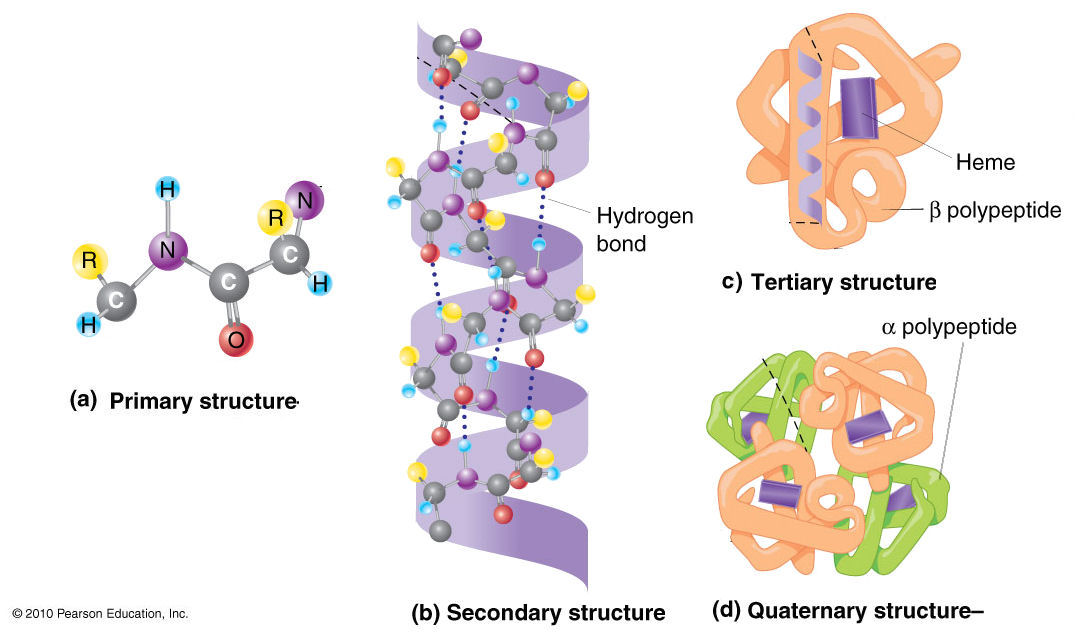
\includegraphics[width=10cm]{img/papers/protein_structure}
		\caption{Types of protein structures. Source: \cite{russell2002igenetics}.}
	\end{figure}
	
\end{frame}
%-------------------------------------------------------
%-------------------------------------------------------

%-------------------------------------------------------
%-------------------------------------------------------
\begin{frame}{Protein structure}{SARS-CoV-2}	
	
	\begin{figure}
		\centering
		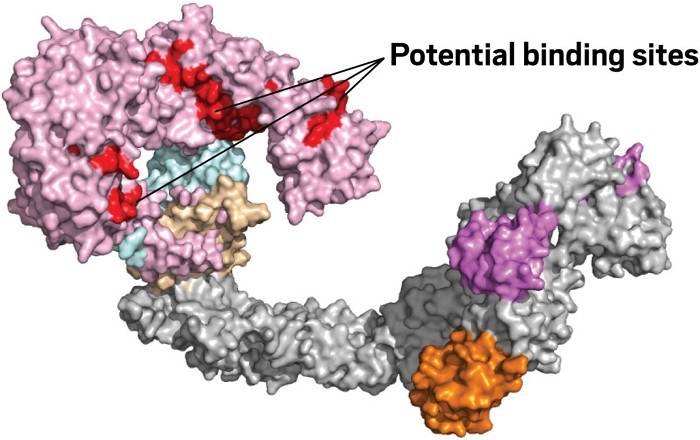
\includegraphics[width=10cm]{img/papers/covid_protein}
		\caption{Example of SARS-CoV-2 protein structure. Source: \chref{https://cen.acs.org/articles/98/i12/es-El-mapeo-de-protenas-encuentra-69-potenciales.html?PageSpeed=noscript}{CEn}.}
	\end{figure}
	
\end{frame}
%-------------------------------------------------------
%-------------------------------------------------------


%-------------------------------------------------------
%-------------------------------------------------------
\begin{frame}{Numbers}{}

	\begin{block}{}
		Protein structures are complex systems with several tens, hundreds and \textbf{thounsand} of residues (amino acids).	
	\end{block}	

	\begin{block}{}
		Only about \textbf{1\%} of the total number of sequenced proteins has experimentally determined. \cite{rangwala2011introduction}.
	\end{block}	

\end{frame}
%-------------------------------------------------------
%-------------------------------------------------------

%-------------------------------------------------------
%-------------------------------------------------------
\begin{frame}{Protein structure prediction}{}
	
	\begin{figure}
		\centering
		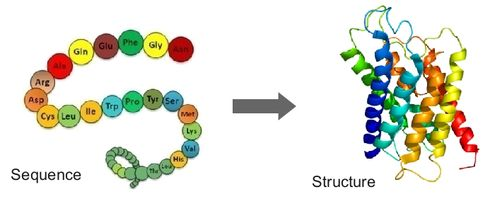
\includegraphics[width=10cm]{img/papers/protein_structure_prediction}
		%\caption{Example of SARS-CoV-2 protein structure. Source: \chref{https://cen.acs.org/articles/98/i12/es-El-mapeo-de-protenas-encuentra-69-potenciales.html?PageSpeed=noscript}{CEn}.}
	\end{figure}
	
\end{frame}
%-------------------------------------------------------
%-------------------------------------------------------


%%%%%%%%%%%%%%%%%%%%%%%%%%%%%%%%%%%%%%%%%%%%%%%%%%%%%%%%%%%%%%%%%%%%%%%%%%%%%%%%%%%%%%%%%%%%%%%%%%%%%%%%%%%%%%%%
%%%%%%%%%%%%%%%%%%%%%%%%%%%%%%%%%%%%%%%%%%%%%%%%%%%%%%%%%%%%%%%%%%%%%%%%%%%%%%%%%%%%%%
\section{Proposal}
%%%%%%%%%%%%%%%%%%%%%%%%%%%%%%%%%%%%%%%%%%%%%%%%%%%%%%%%%%%%%%%%%%%%%%%%%%%%%%%%%%%%%%%%%%%%%%%%%%%%%%%%%%%%%%%%
%%%%%%%%%%%%%%%%%%%%%%%%%%%%%%%%%%%%%%%%%%%%%%%%%%%%%%%%%%%%%%%%%%%%%%%%%%%%%%%%%%%%%%

%%%%%%%%%%%%%%%%%%%%%%%%%%%%%%%%%%%%%%%%%%%%%%%%%%%%%%%%%%%%%%%%%%%%%%%%%%%%%%%%%%%%%%%%%%%%%%%%%%%%%%%%%%%%%%%%
%%%%%%%%%%%%%%%%%%%%%%%%%%%%%%%%%%%%%%%%%%%%%%%%%%%%%%%%%%%%%%%%%%%%%%%%%%%%%%%%%%%%%%
\subsection{Protein structure prediction}
%%%%%%%%%%%%%%%%%%%%%%%%%%%%%%%%%%%%%%%%%%%%%%%%%%%%%%%%%%%%%%%%%%%%%%%%%%%%%%%%%%%%%%%%%%%%%%%%%%%%%%%%%%%%%%%%
%%%%%%%%%%%%%%%%%%%%%%%%%%%%%%%%%%%%%%%%%%%%%%%%%%%%%%%%%%%%%%%%%%%%%%%%%%%%%%%%%%%%%%

%-------------------------------------------------------
%-------------------------------------------------------
\begin{frame}{Protein structure prediction}{}
	
	\begin{block}{}
		\centering
		\textbf{DESTINI: A deep-learning approach to contact-driven protein structure prediction} \cite{gao2019destini}.
	\end{block}
	
	\begin{itemize}
		\item \textbf{Year}: 2019
		\item \textbf{Authors}: Gao, Mu and Zhou, Hongyi and Skolnick, Jeffrey
		\item \textbf{Event}: Journal of Scientific reports
	\end{itemize}
\end{frame}
%-------------------------------------------------------
%-------------------------------------------------------

%-------------------------------------------------------
%-------------------------------------------------------
\begin{frame}{Protein structure prediction}{}
	\begin{figure}
		\centering
		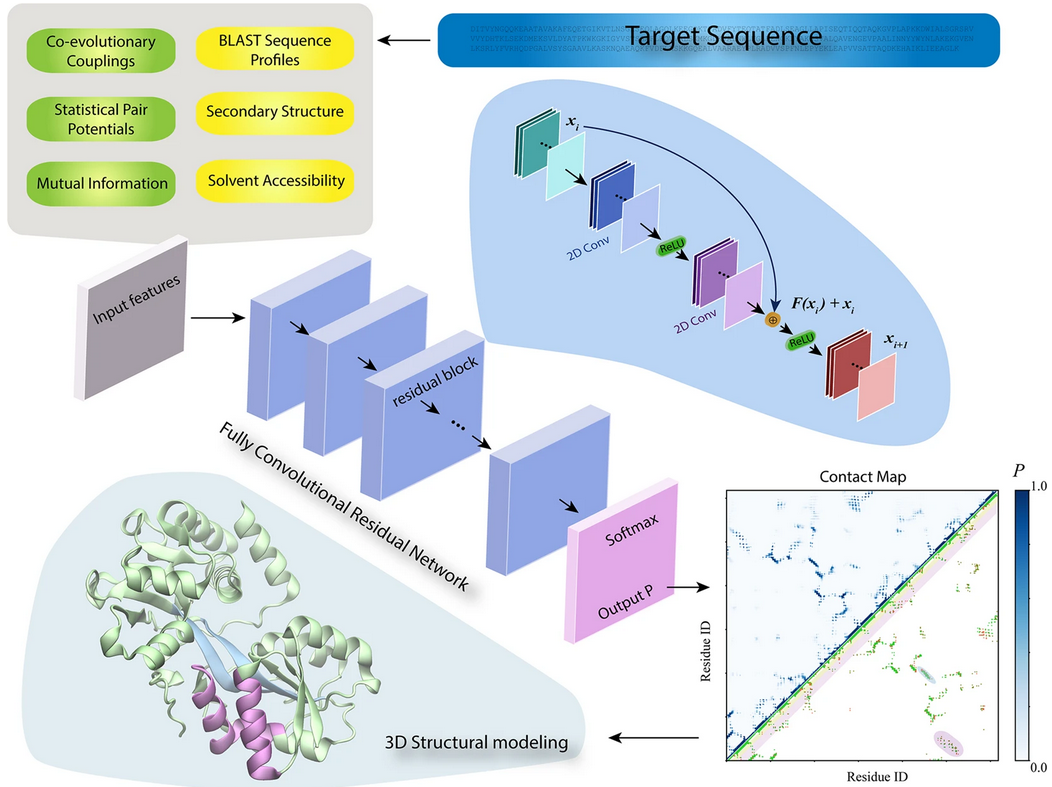
\includegraphics[width=10cm]{img/papers/paper4}
		\caption{Pipeline for 3D protein structure prediction using deep learning. Source: \cite{ando2020practical}.}
	\end{figure}
\end{frame}
%-------------------------------------------------------
%-------------------------------------------------------


%%%%%%%%%%%%%%%%%%%%%%%%%%%%%%%%%%%%%%%%%%%%%%%%%%%%%%%%%%%%%%%%%%%%%%%%%%%%%%%%%%%%%%%%%%%%%%%%%%%%%%%%%%%%%%%%
%%%%%%%%%%%%%%%%%%%%%%%%%%%%%%%%%%%%%%%%%%%%%%%%%%%%%%%%%%%%%%%%%%%%%%%%%%%%%%%%%%%%%%
\subsection{Contact map}
%%%%%%%%%%%%%%%%%%%%%%%%%%%%%%%%%%%%%%%%%%%%%%%%%%%%%%%%%%%%%%%%%%%%%%%%%%%%%%%%%%%%%%%%%%%%%%%%%%%%%%%%%%%%%%%%
%%%%%%%%%%%%%%%%%%%%%%%%%%%%%%%%%%%%%%%%%%%%%%%%%%%%%%%%%%%%%%%%%%%%%%%%%%%%%%%%%%%%%%

%-------------------------------------------------------
%-------------------------------------------------------
\begin{frame}{Contact map}{3D model from contact map}
	\begin{figure}
		\centering
		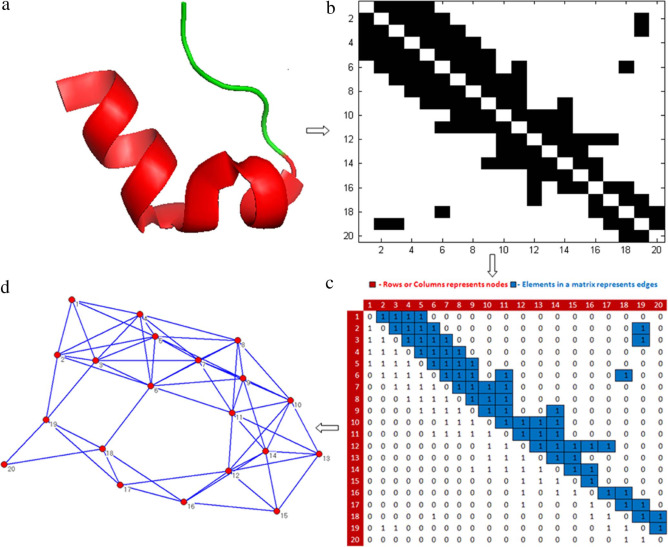
\includegraphics[width=8cm]{img/papers/contact_map}
		\caption{Contact map derive from 3D protein model. Source: \cite{emerson2017protein}.}
	\end{figure}
\end{frame}
%-------------------------------------------------------
%-------------------------------------------------------

%-------------------------------------------------------
%-------------------------------------------------------
\begin{frame}{Contact map}{3D model from contact map}
	\begin{block}{}
		Reconstruct a 3D protein model from the contact map is challenging \cite{emerson2017protein}.
	\end{block}

	\begin{block}{}
		Methods are divided into \textit{ad initio} and template-based \cite{emerson2017protein}.
	\end{block}
\end{frame}
%-------------------------------------------------------
%-------------------------------------------------------


%-------------------------------------------------------
%-------------------------------------------------------
\begin{frame}{3D reconstruction}{Protein structure Modeling}
	
	\begin{block}{}
		\centering
		\textbf{Reconstruction of 3D Structures from Protein Contact Maps} \cite{vassura2008reconstruction}.
	\end{block}
	
	\begin{itemize}
		\item \textbf{Year}: 2008
		\item \textbf{Authors}: Transactions on Computational Biology and Bioinformatics
		\item \textbf{Event}: BMC Bioinformatics
	\end{itemize}
\end{frame}
%-------------------------------------------------------
%-------------------------------------------------------


%-------------------------------------------------------
%-------------------------------------------------------
\begin{frame}{CONFOLD2}{Protein structure Modeling}
	
	\begin{block}{}
		\centering
		\textbf{CONFOLD2: improved contact-driven ab initio protein structure modeling} \cite{adhikari2018confold2}.
	\end{block}
	
	\begin{itemize}
		\item \textbf{Year}: 2018
		\item \textbf{Authors}: Adhikari, Badri and Cheng, Jianlin
		\item \textbf{Event}: BMC Bioinformatics
	\end{itemize}
\end{frame}
%-------------------------------------------------------
%-------------------------------------------------------

%%%%%%%%%%%%%%%%%%%%%%%%%%%%%%%%%%%%%%%%%%%%%%%%%%%%%%%%%%%%%%%%%%%%%%%%%%%%%%%%%%%%%%%%%%%%%%%%%%%%%%%%%%%%%%%%
%%%%%%%%%%%%%%%%%%%%%%%%%%%%%%%%%%%%%%%%%%%%%%%%%%%%%%%%%%%%%%%%%%%%%%%%%%%%%%%%%%%%%%
\subsection{Deep learning}
%%%%%%%%%%%%%%%%%%%%%%%%%%%%%%%%%%%%%%%%%%%%%%%%%%%%%%%%%%%%%%%%%%%%%%%%%%%%%%%%%%%%%%%%%%%%%%%%%%%%%%%%%%%%%%%%
%%%%%%%%%%%%%%%%%%%%%%%%%%%%%%%%%%%%%%%%%%%%%%%%%%%%%%%%%%%%%%%%%%%%%%%%%%%%%%%%%%%%%%

%-------------------------------------------------------
%-------------------------------------------------------
\begin{frame}{DMPfold}{Protein structure Prediction}
	
	\begin{block}{}
		\centering
		\textbf{Deep learning extends de novo protein modelling coverage of genomes using iteratively predicted structural constraints} \cite{greener2019deep}.
	\end{block}
	
	\begin{itemize}
		\item \textbf{Year}: 2019
		\item \textbf{Authors}: Greener, Joe G and Kandathil, Shaun M and Jones, David T
		\item \textbf{Event}: Nature communications
		\item \textbf{Repository}: \chref{https://github.com/psipred/DMPfold}{git} 
	\end{itemize}
\end{frame}
%-------------------------------------------------------
%-------------------------------------------------------


%-------------------------------------------------------
%-------------------------------------------------------
\begin{frame}{AlphaFold}{Protein structure Prediction}
	
	\begin{block}{}
		\centering
		\textbf{Protein structure prediction using multiple deep neural networks in the 13th Critical Assessment of Protein Structure Prediction (CASP13)} \cite{senior2019protein}.
	\end{block}
	
	\begin{itemize}
		\item \textbf{Year}: 2019
		\item \textbf{Authors}: Senior, Andrew W and Evans, ...
		\item \textbf{Event}: CASP13
	\end{itemize}
\end{frame}
%-------------------------------------------------------
%-------------------------------------------------------

%-------------------------------------------------------
%-------------------------------------------------------
\begin{frame}[allowframebreaks]
	\frametitle{References}
	%\bibliographystyle{amsalpha}
	\bibliographystyle{IEEEtran}
	\bibliography{bibliography.bib}
\end{frame}
%-------------------------------------------------------
%-------------------------------------------------------


%-------------------------------------------------------
%-------------------------------------------------------
\if\mycmd1 % MY THEME
\1{
	{\1
		\begin{frame}[plain,noframenumbering]
			%\finalpage{Thank you}
			\begin{figure}[]
				\centering
				
\includegraphics[width=\textwidth,height=0.7\textheight,keepaspectratio]{img/question.png}
				%\label{img:mot2}
				%\caption{Image example in 2 gray levels.}
			\end{figure}
	\end{frame}}
	\else % CS THEME
	\begin{frame}{Questions?}
		\begin{figure}[]
			\centering
			
\includegraphics[width=\textwidth,height=0.7\textheight,keepaspectratio]{img/question.png}
			%\label{img:mot2}
			%\caption{Image example in 2 gray levels.}
		\end{figure}
		
	\end{frame}
	\fi
	%-------------------------------------------------------
	%-------------------------------------------------------
	

\end{document}